\section{Ontwerp studie}
Om een objectief beeld te krijgen van de effectiviteit van mijn implementatie van
change blindness heb ik een simpel experiment opgesteld. Elke testpersoon kreeg
een briefing waar hem verteld werd dat hij door een virtueel kantoor zou gaan
wandelen. Ik deelde hem mee dat hij in elk kantoor de blinden zou moeten sluiten 
met de knop naast het raam, en dat hij de foto boven deze knop moest onthouden.
Vervolgens werd hem gevraagd het kantoor te verlaten en de deur achter hem te
sluiten en dit proces voor 3 kantoren te herhalen. Er werd ook kort aan de 
proefpersonen verteld hoe ze moesten interageren met de virtuele omgeving.

Vervolgens werd er gevraagd of er onduidelijkheden waren en begaven we ons naar 
de startpositie, en werd de proefpersoon de Oculus Rift aangeboden om zelf op te 
zetten.

Na de uitvoering van het experiment werd de proefpersoon een korte vragenlijst
voorgelegd.


\subsection{Vragenlijst}
De vragenlijst bestond uit een informatieblok en vijf vragen. Ze was beschikbaar
in het Nederlands en het Engels.

In het informatieblok wordt er gevraagd naar de leeftijd en het geslacht van de
proefpersoon, dit om potentieel te analyseren of er verschillen in effectiviteit
tussen deze groepen zijn.

Vervolgens wordt er gevraagd om een schema van het grondplan te tekenen, om te
zien of er ondanks de onmogelijke ruimte toch een consistent mentaal beeld kon
gevormd worden. Daarna wordt er gevraagd om de drie fotos op te noemen, maar 
dit is irrelevant en dient enkel als afleiding.

In vraag drie moet de proefpersoon aan acht stellingen een score toekennen van 1
tot 6 waar 1 betekent dat hij het niet heeft gemerkt, en 6 dat heel duidelijk wel 
is gebeurd:

\begin{enumerate}
  \item Ik zag de virtuele omgeving groter of kleiner worden.
  \item \emph{Ik voelde alsof ik het zelfde pad aan het belopen was.}
  \item Ik zag de virtuele omgeving flitsen.
  \item \emph{Ik merkte dat iets in de omgeving zich van plaats had veranderd.}
  \item Ik zag de virtuele omgeving roteren.
  \item Ik voelde mezelf groter of kleiner worden.
  \item Ik voelde me alsof ik bewogen werd.
  \item Ik merkte dat iets in de virtuele omgeving groter of kleiner werd.
\end{enumerate}

Enkel de schuingedrukte stellingen zijn echt gebeurd, de andere stellingen zouden
een zeer lage gemiddelde score moeten hebben.

De laatste twee vragen bestaan uit een vraag waar wordt gevraagd voor algemene
qualitatieve feedback over de immersie, en een vraag waar wordt gevraagd om de 
bewogen voorwerpen te identificeren.

De vragenlijst is gedeeltelijk overgenomen van de vragenlijst uit het experiment
van Evan A. Suma\cite{suma11}.


\section{Uitvoering}
Het experiment is uitgevoerd met 17 proefpersonen, 4 vrouwen en 13 mannen.
Leeftijden varieerden van 21 tot 47 jaar oud met een gemiddelde van 30. Slechts
3 personen hadden geen spelervaring. Omdat zowel de groep van vrouwen als de
groep van mensen zonder spelervaring te klein is kunnen deze groepen helaas
niet apart bekeken worden.


\section{Bespreking data}
De geleverde grondplannen kwamen over het algemeen overeen met de realiteit, de
enige uitzondering hier op was het grondplan van proefpersoon 17, zijn kaart was
gespiegeld over de as die met de gang mee loopt.

\begin{figure}[p]
    \centering
    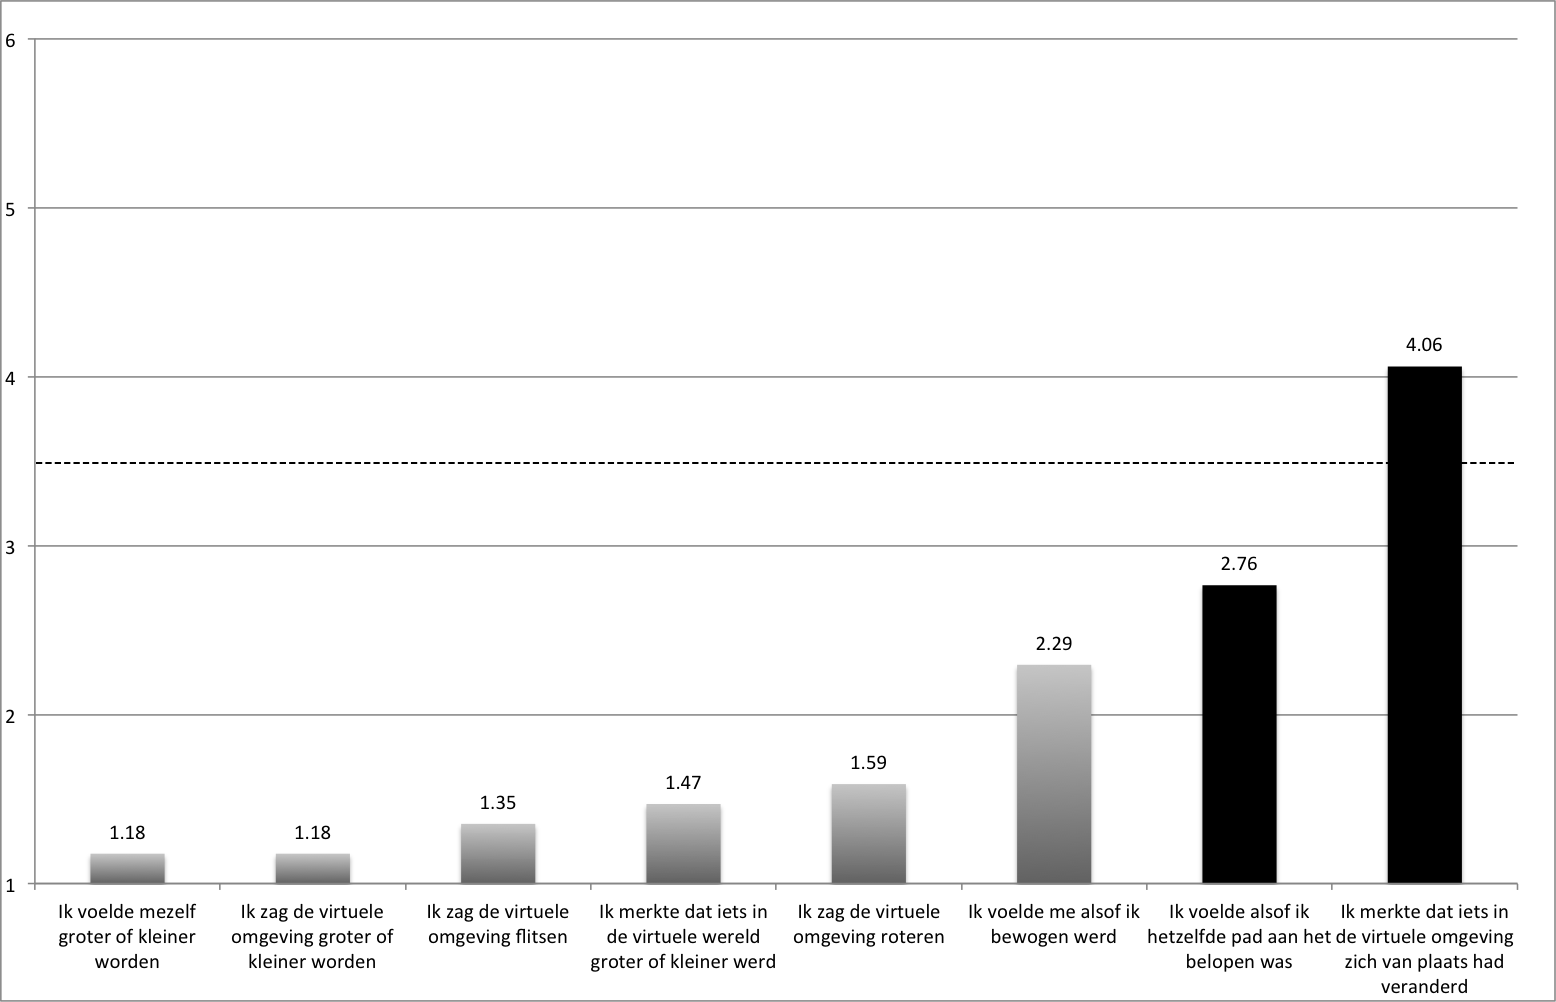
\includegraphics[width=\textwidth]{chart}
    \caption{Grafiek van de gemiddelde scores van de stellingen, de zwarte 
    kolommen zijn de ware stellingen.}
    \label{fig:chart}
\end{figure}

\begin{figure}[p]
    \centering
    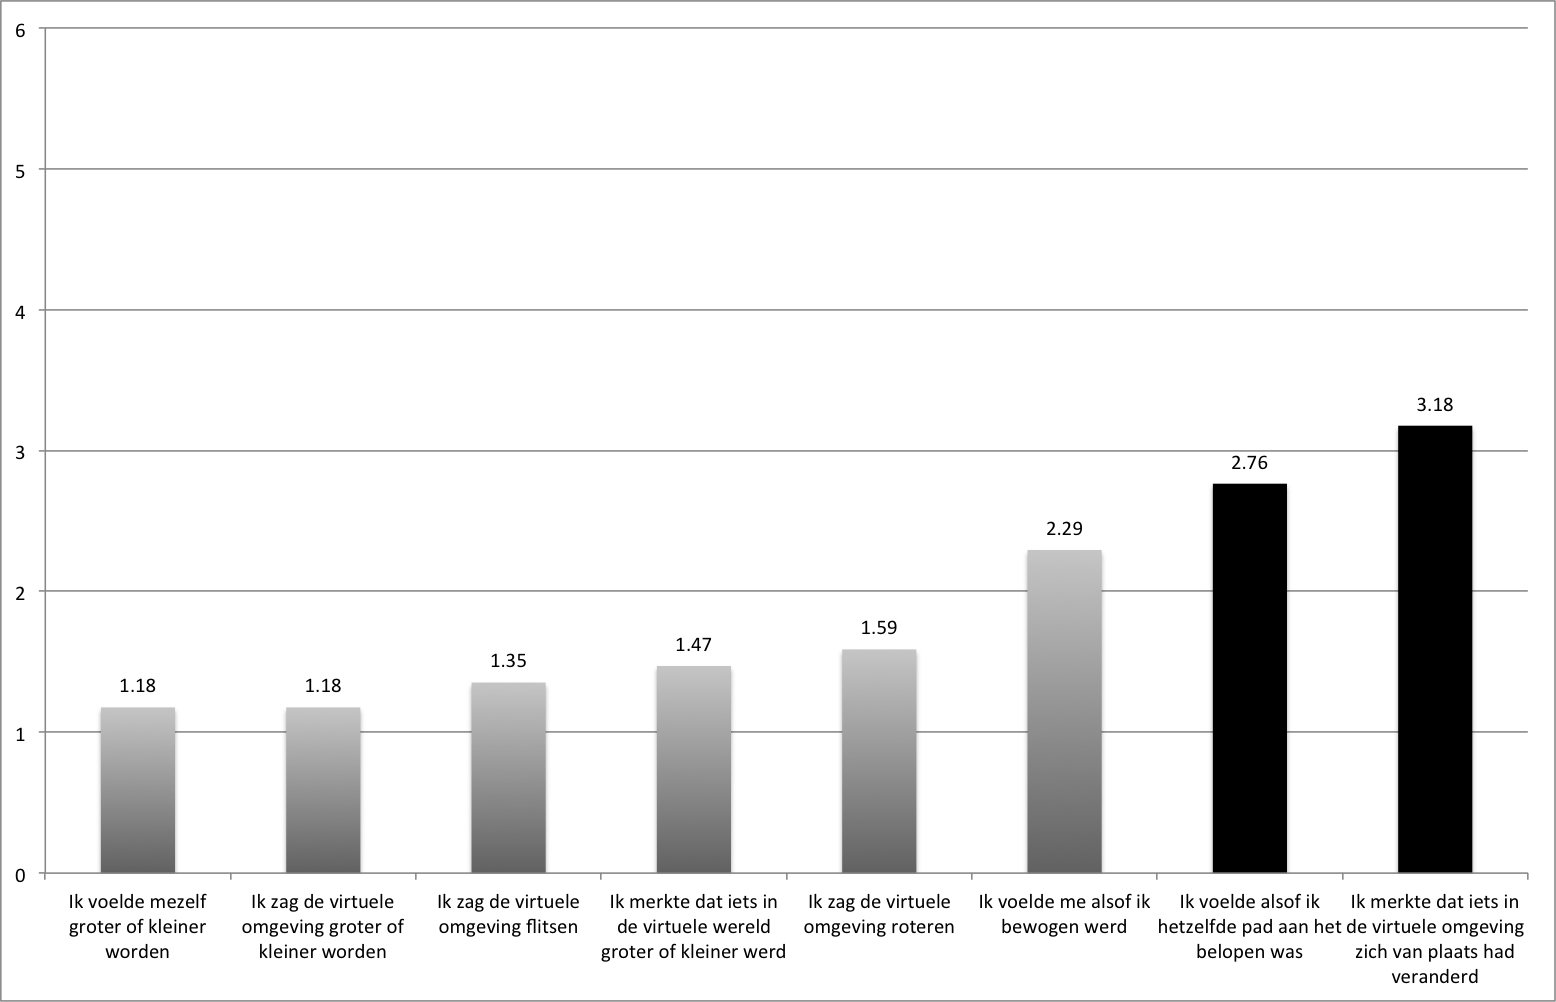
\includegraphics[width=\textwidth]{chartmod}
    \caption{Grafiek van de gemiddelde scores van de stellingen, de zwarte 
    kolommen zijn de ware stellingen. De gegeven scores van de mensen die het
    bewogen object niet correct konden identificeren zijn naar ``1'' aangepast.}
    \label{fig:chartmod}
\end{figure}

Scores voor de afleidingsstellingen vari\"eren tussen 1.18 en 2.29, de hoge score
van ``Ik voelde me alsof ik bewogen werd'' valt hier op. Vermoedelijk werd die
vraag door sommigen verkeerd ge\"interpreteerd of had mijn aanwezigheid in de
tracking area hier mee te maken.

Zowel ``Ik voelde alsof ik hetzelfde pad aan het belopen was'' ($\bar{x}$: 2.76)
als ``Ik voelde alsof ik hetzelfde pad aan het belopen was'' ($\bar{x}$: 4.06)
behaalden zeer hoge gemiddelde scores. Indien ik de scores van de personen die
het bewegen van de deur niet correct konden identificeren naar ``1'' laat zakken
verlaagt deze laatste score tot $\bar{x}$: 3.18.

Hoewel deze aanpassing een lagere score teweeg brengt is deze nog steeds
voldoende hoog om te concluderen dat deze specifieke implementatie van
change blindness niet goed werkt op deze specifieke groep van proefpersonen.

Ondanks dit resultaat heeft het toch gewerkt op meer dan de helft van de
testgroep, 53\% van de testgroep merkte de verplaatsing van de deuren niet.


\section{Bespreking feedback}
Een van de vragen op de vragenlijst vroeg of er iets was dat de immersie breekt.
Er werd hier feedback gegeven op diverse problemen:

\begin{itemize}
  \item Fysieke problemen zoals de grootte van de Oculus Rift, het storen van de
        kabels, en rakelings tegen het doek lopen.
  \item Technische problemen zoals het ontbreken van een realistisch input device
        en de resolutie van de Oculus Rift.
\end{itemize}

Als laatste heb ik ook feedback gekregen dat er kleine haperingen in de tracking
waren, helaas zijn deze kleine haperingen veroorzaakt door een onvoldoende aantal
cameras en kon ik hier niets aan doen. Wegens een kleine hoeveelheid 
netwerklatency zat er ook een beetje lag op de reactiesnelheid van het systeem. 
Een van de proefpersonen was ook te groot voor de tracking setup en moest een
beetje gebukt door de omgeving lopen. Enkele van de proefpersonen die de 
verplaatsing van de deur merkten noteerden dit ook als immersiebrekend.